\documentclass[10pt,dvipdfmx]{beamer}
\usepackage{pxjahyper}% しおりの文字化け対策
\usepackage{minijs}% 和文メトリック
\renewcommand{\kanjifamilydefault}{\gtdefault}%ゴシックにする
\setbeamertemplate{navigation symbols}{}%dvipdfmxではナビゲーションシンボルが機能しないので除去

\usepackage{pxghost}
\makeatletter
\def\verbstart{{\pxqgg@TI\pxqgg@cwm}\verb}
\def\verbend{{\pxqgg@TI\pxqgg@cwm}}
\makeatother
\usepackage{mhchem}
\graphicspath{{./img/}}
\def\sankazai{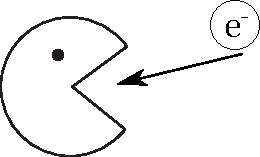
\includegraphics[width=1cm]{./sankazai.pdf}}
\def\kangenzai{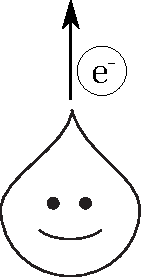
\includegraphics[width=0.5cm]{./kangenzai.pdf}}
\def\cto{\ \rightarrow\ }
\def\ceq{\ \leftrightarrows\ }
\def\穴#1{\pause\alert{#1}\pause}
\usepackage{amssymb,amsmath,ascmac}

\usetheme{Warsaw}
\usefonttheme{professionalfonts}

\title[beamer入門&正規表現]{beamerを使って授業プリントをそのままスライド化!/正規表現}
\author[domperor]{domperor}
\institute[UT-TeX/Tetsuryokukai]{UT-TeX-Club/Tetsuryokukai}
\date{Sep 2.}


\begin{document}
\maketitle

\section{なぜbeamerか}
%%%%%%%%%%%% シートstart %%%%%%%%%%%%
\begin{frame}[t]
 \frametitle{なぜbeamerか}

\begin{enumerate}
\item もともと\LaTeX で本文を打ち込んだなら,それをそのままソースとして使える
\item やはり\TeX 愛好会としてはスライドも\LaTeX じゃなきゃ\item なお,tetsuryoku.sty/tetsuchem.sty/jsclassesとの共存は厳しいです……(コマンドで必要なものがあればstyからコピペするか作りましょう)
\end{enumerate}

\hangindent1em
※このbeamerサンプルファイルはあべのりさんのをベースに書いています。多謝。

\url{https://www.ms.u-tokyo.ac.jp/~tado/beamer/}

\ 

\hangindent1em
※Referenceファイルはこれがわかりやすい。\alert{←使いながら実習}

\url{http://ayapin-film.sakura.ne.jp/LaTeX/Slides/Beamer-tutorial.pdf}

\end{frame}
%%%%%%%%%%%% シートend %%%%%%%%%%%%


%%%%%%%%%%%% シートstart %%%%%%%%%%%%
\begin{frame}[c,fragile]
\frametitle{穴埋めプリントをそのままスライド化できる!}
\begin{block}{元々のソースはこんな感じ}
\small
\begin{verbatim}
\begin{itemize}
\item \sankazai \ce{F2},\ce{Cl2},\ce{Br2},\ce{I2}を酸化力順に並べると……\穴{\ce{F2},\ce{Cl2},\ce{Br2},\ce{I2}}
\item \ce{F2}と\ce{H2O}の化学反応式:
\穴{\ce{2F2 + 2H2O $\cto$ 4HF + O2}}
\item \ce{Cl2}と\ce{H2O}の化学反応式:
\穴{\ce{Cl2 + H2O $\ceq$ HCl + HClO}}
\item \ce{Cl2}の製法1つ目(化学反応式):
\穴{\ce{MnO2 + 4HCl ->C[\Delta][] MnCl2 + 2H2O + Cl2}}
\item \ce{Cl2}の製法2つ目(化学反応式):
\穴{\ce{CaCl(ClO).H2O + 2HCl -> CaCl2 + 2H2O + Cl2}}
\end{itemize}
\end{verbatim}
\end{block}
\end{frame}
%%%%%%%%%%%% シートend %%%%%%%%%%%%


%%%%%%%%%%%% シートstart %%%%%%%%%%%%
\begin{frame}[c,fragile]
\frametitle{そのままのソースで,出来上がりはこうなる}
\begin{itemize}
\item \sankazai \ce{F2},\ce{Cl2},\ce{Br2},\ce{I2}を酸化力順に並べると……\穴{\ce{F2},\ce{Cl2},\ce{Br2},\ce{I2}}
\item \ce{F2}と\ce{H2O}の化学反応式:
\穴{\ce{2F2 + 2H2O $\cto$ 4HF + O2}}
\item \ce{Cl2}と\ce{H2O}の化学反応式:
\穴{\ce{Cl2 + H2O $\ceq$ HCl + HClO}}
\item \ce{Cl2}の製法1つ目(化学反応式):
\穴{\ce{MnO2 + 4HCl ->C[\Delta][] MnCl2 + 2H2O + Cl2}}
\item \ce{Cl2}の製法2つ目(化学反応式):
\穴{\ce{CaCl(ClO).H2O + 2HCl -> CaCl2 + 2H2O + Cl2}}
\end{itemize}
\end{frame}
%%%%%%%%%%%% シートend %%%%%%%%%%%%

%%%%%%%%%%%% シートstart %%%%%%%%%%%%
\begin{frame}[c,fragile]
\frametitle{スライドに落とし込む上で解決すべき問題点}
(1)mhchemパッケージの読み込み

(2)独自命令\,\verbstart|\sankazai|\verbend 

(3)鉄緑命令\,\verbstart|\cto|\verbend ・\verbstart|\ceq|\verbend 

(4)「\verbstart|\穴|\verbend 」の挙動
\end{frame}
%%%%%%%%%%%% シートend %%%%%%%%%%%%

%%%%%%%%%%%% シートstart %%%%%%%%%%%%
\begin{frame}[c,fragile]
 \frametitle{(1)パッケージの読み込み,(2)独自命令}
 \begin{itemize}
\item (鉄緑事情)普段,tetsuryoku.sty/tetsuchem.styだけ読み込んでいれば必要かもしれないパッケージは全て一括で読み込んでくれるようになっている。
\item それを封じられたので,必要な命令ごとにパッケージを読み込む必要がある。(一般ユーザはこれが普通)
\item たとえば\verbstart|\ce|\verbend 命令はmhchemパッケージが提供するので,\verbstart|\usepackage{mhchem}|\verbend 
\item 他にも,自分で定義した独自命令の移植をお忘れなく

(例:\verbstart|\def\sankazai{\includegraphics[width=1cm]|\verbend

\hfill\verbstart|{./sankazai.pdf}}|\verbend )
 \end{itemize}
\end{frame}
%%%%%%%%%%%% シートend %%%%%%%%%%%%

%%%%%%%%%%%% シートstart %%%%%%%%%%%%
\begin{frame}[c,fragile]
\frametitle{(3)鉄緑命令/jsclasses命令}
\begin{itemize}
\item \verbstart|\cto|\verbend ・\verbstart|\ceq|\verbend などtetsuryoku/tetsuchem独自の命令や,\verbstart|\aj|\verbend で始まるjsclasses独自の命令を使いたいときは,対処が必要。
\item \verbstart|\cto|\verbend ・\verbstart|\ceq|\verbend は\verbstart|\rightarrow|\verbend ・\verbstart|\leftrightarrows|\verbend ,\verbstart|\ajMaru{カウンタ}|\verbend は\verbstart|\circled{〜}|\verbend など一般的な命令に変わるように配慮する。
\item 例えばプリアンブルで次のように定義してしまえばよかろう。最初はちょっと面倒な作業だが,一度やってしまえば2度とやる必要はない。
\end{itemize}
\begin{block}{ローカルルール命令を一般的なものに置き換え}
\small
\begin{verbatim}
\def\cto{\ \rightarrow\ }
\def\ceq{\ \leftrightarrows\ }
\end{verbatim}
\end{block}
\end{frame}
%%%%%%%%%%%% シートend %%%%%%%%%%%%

%%%%%%%%%%%% シートstart %%%%%%%%%%%%
\begin{frame}[c,fragile]
\frametitle{(4)「\textbackslash 穴」の挙動}
普通の穴埋めプリントでは,次のようにテキスト色を変えることで講師用と生徒用を使い分ける方法が主流か。

\begin{block}{元々のソースはこんな感じ}
\small
\begin{verbatim}
\def\ステータス{生徒用}%切り替える
%\def\ステータス{講師用}%切り替える
\ifthenelse{\equal{\ステータス}{講師用}}{\def\穴埋め色{red}}{\def\穴埋め色{white}}
\def\穴#1{\下線{\textcolor{\穴埋め色}{#1}}}
\end{verbatim}
\end{block}
生徒用,講師用コンパイルの様子

\mbox{}\kern-3em
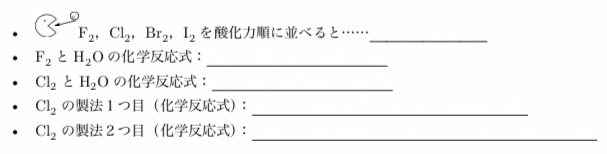
\includegraphics[width=0.6\linewidth]{生徒用コンパイル.png}\nobreak
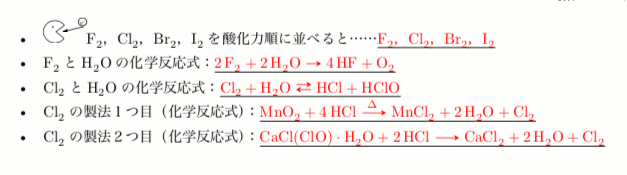
\includegraphics[width=0.6\linewidth]{講師用コンパイル.png}
\end{frame}
%%%%%%%%%%%% シートend %%%%%%%%%%%%

%%%%%%%%%%%% シートstart %%%%%%%%%%%%
\begin{frame}[c,fragile]
\frametitle{(4)「\textbackslash 穴」の挙動}
スライドショーでは,答えが隠れていて,一回押すと答えが見えるようになるのが主流か。\Large\verbstart|\pause|\verbend 機能と\verbstart|\alert|\verbend 機能を使いこなそう。\normalsize

\begin{block}{スライド用ソースはたったこれだけ}
\small
\begin{verbatim}
\def\穴#1{\pause\alert{#1}\pause}
\end{verbatim}
\end{block}

→もう一回見てみましょう
\end{frame}
%%%%%%%%%%%% シートend %%%%%%%%%%%%

%%%%%%%%%%%% シートstart %%%%%%%%%%%%
\begin{frame}[c,fragile]
\frametitle{こうなります}
\begin{itemize}
\item \sankazai \ce{F2},\ce{Cl2},\ce{Br2},\ce{I2}を酸化力順に並べると……\穴{\ce{F2},\ce{Cl2},\ce{Br2},\ce{I2}}
\item \ce{F2}と\ce{H2O}の化学反応式:
\穴{\ce{2F2 + 2H2O $\cto$ 4HF + O2}}
\item \ce{Cl2}と\ce{H2O}の化学反応式:
\穴{\ce{Cl2 + H2O $\ceq$ HCl + HClO}}
\item \ce{Cl2}の製法1つ目(化学反応式):
\穴{\ce{MnO2 + 4HCl ->C[\Delta][] MnCl2 + 2H2O + Cl2}}
\item \ce{Cl2}の製法2つ目(化学反応式):
\穴{\ce{CaCl(ClO).H2O + 2HCl -> CaCl2 + 2H2O + Cl2}}
\end{itemize}
\end{frame}
%%%%%%%%%%%% シートend %%%%%%%%%%%%


%%%%%%%%%%%% シートstart %%%%%%%%%%%%
\begin{frame}[c,fragile]
 \frametitle{他の色付け}
  {\color{red} red}(\alert{alert}),
  {\color{blue} blue}(\structure{structure}),
  {\color{green} green},
  {\color{cyan} cyan},
  {\color{magenta} magenta},
  {\color{yellow} yellow},
  {\color{black} black},
  {\color{darkgray} darkgray},
  {\color{gray} gray},
  {\color{lightgray} lightgray},
  {\color{orange} orange},
  {\color{violet} violet},
  {\color{purple} purple},
  {\color{brown} brown},
\end{frame}
%%%%%%%%%%%% シートend %%%%%%%%%%%%

%%%%%%%%%%%% シートstart %%%%%%%%%%%%
\begin{frame}[c,fragile]
 \frametitle{他のタイミングで出したり隠したり}
\begin{itemize}
\item<1,3> \sankazai \ce{F2},\ce{Cl2},\ce{Br2},\ce{I2}を酸化力順に並べると……\alert{\ce{F2},\ce{Cl2},\ce{Br2},\ce{I2}}
\item<2,3> \ce{F2}と\ce{H2O}の化学反応式:
\alert{\ce{2F2 + 2H2O $\cto$ 4HF + O2}}
\item<1,3> \ce{Cl2}と\ce{H2O}の化学反応式:
\alert{\ce{Cl2 + H2O $\ceq$ HCl + HClO}}
\item<2,3> \ce{Cl2}の製法1つ目(化学反応式):
\alert{\ce{MnO2 + 4HCl ->C[\Delta][] MnCl2 + 2H2O + Cl2}}
\item<1,3> \ce{Cl2}の製法2つ目(化学反応式):
\alert{\ce{CaCl(ClO).H2O + 2HCl -> CaCl2 + 2H2O + Cl2}}
\end{itemize}
\end{frame}
%%%%%%%%%%%% シートend %%%%%%%%%%%%


%%%%%%%%%%%% シートstart %%%%%%%%%%%%
\begin{frame}[t]
 \frametitle{コラム}
  \begin{columns}[t]
   \begin{column}{.3\textwidth}
    他の機能はやはり最初に述べた通り→のドキュメントが詳しいです。ダウンロードして持っておきましょう。
    \begin{itemize}
\item beamercolorbox
\item columns環境
\item 表示時期指定子の詳細
\item 表/図/TikZ
\item ハイパーリンク
\item フォント
\end{itemize}
   \end{column}
   \begin{column}{.4\textwidth}
    \begin{alertblock}{URL}
     \url{http://ayapin-film.sakura.ne.jp/LaTeX/Slides/Beamer-tutorial.pdf}
    \end{alertblock}
   \end{column}
  \end{columns}
\end{frame}
%%%%%%%%%%%% シートend %%%%%%%%%%%%


\section{正規表現}
%%%%%%%%%%%% シートstart %%%%%%%%%%%%
\begin{frame}[t]
 \frametitle{正規表現}

ここからはbeamer全く関係ないです。TeXShop,TeXWorks,TeXStudioなどのメジャーなエディタには正規表現一括置換が備わっています。これを使いこなせるとつよいよね!というお話。

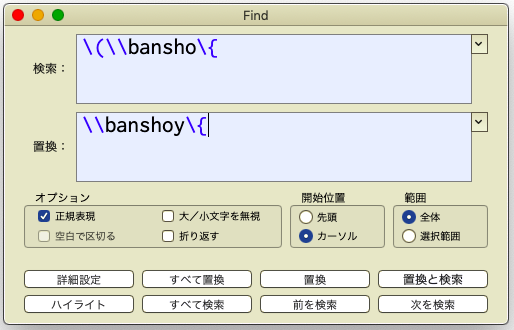
\includegraphics[width=0.6\linewidth]{TeXShop一括置換画面.png}

他のプログラミング言語を触る時でも,\alert{正規表現はめっちゃ重要で基本技能の一つ}に数えられるだろう。

\quad 例:Python ではimport reで正規表現のモジュールが読み込める
\end{frame}
%%%%%%%%%%%% シートend %%%%%%%%%%%%

%%%%%%%%%%%% シートstart %%%%%%%%%%%%
\begin{frame}[t]
 \frametitle{正規表現レファレンス}
 
例もあってみやすいものを。

\begin{itemize}
\item 基本的なものに絞ったリスト

\url{https://murashun.jp/blog/20190215-01.html}

\item 肯定先読み/否定先読みまで含めた詳細なリスト

\url{https://www.megasoft.co.jp/mifes/seiki/meta.html}
\end{itemize}

\end{frame}
%%%%%%%%%%%% シートend %%%%%%%%%%%%

%%%%%%%%%%%% シートstart %%%%%%%%%%%%
\begin{frame}[t,fragile]
 \frametitle{練習問題}
 
レファレンスを見つつ,練習問題にトライしてみよう。まずは検索の練習問題。練習用ファイルにおいて何個ヒットするか。

\begin{enumerate}
\item 半角算用数字を検索する
\item アルファベット10文字以上の連続を検索する
\item 「〜」で囲まれたセリフを検索する(最長マッチにならないよう注意!下の例では3つであってほしい。)

\hangindent2em
例)法師は呟いた,「螻蛄は弊れ」,と。吾桑の遺した「7千万回の噯気や」の意味が解ったのである。流離いの軍は間髪を容れず「鍾馗に白檀を」と叫ぶ。

\item 郵便番号を検索
\item 5の倍数だけ検索
\item 冠詞のaのみを検索。aが入る単語ではなく,a1文字で独立している場合だけ検索。
\end{enumerate}

\end{frame}
%%%%%%%%%%%% シートend %%%%%%%%%%%%

%%%%%%%%%%%% シートstart %%%%%%%%%%%%
\begin{frame}[t,fragile]
 \frametitle{練習問題}
レファレンスを見つつ,練習問題にトライしてみよう。次に置換の練習問題。

\begin{enumerate}
\item 行頭にあるbeginを\verbstart|\begin|\verbend にする
\item \verbstart|{{|\verbend 〜\verbstart|}}|\verbend と無駄に二重かっこで囲まれた部分を一重かっこに直す
\item \verbstart|{\color{red}|\verbend 〜\verbstart|}|\verbend の形で書いてある部分を\verbstart|\textcolor{red}{|\verbend 〜\verbstart|}|\verbend の形に直す
\item \verbstart|\下線{|\verbend 〜\verbstart|}|\verbend 中の\verbstart|\ce|\verbend を\verbstart|\uce|\verbend に直す
\item \verbstart|\下線{|\verbend 〜\verbstart|}|\verbend または\verbstart|\強調{|\verbend 〜\verbstart|}|\verbend 中の\verbstart|\ce|\verbend を\verbstart|\uce|\verbend に直す
\item Excelから持ってきた3列の表(Tab&Enterで区切られている)を,\verbstart|{|\verbend 〜\verbstart|}{|\verbend 〜\verbstart|}{|\verbend 〜\verbstart|}|\verbend で区切る
\end{enumerate}

\end{frame}
%%%%%%%%%%%% シートend %%%%%%%%%%%%

%%%%%%%%%%%% シートstart %%%%%%%%%%%%
\begin{frame}[t,fragile]
 \frametitle{検索答え}

\begin{enumerate}
\item 半角算用数字を検索する:\alert{45個}

{\color{blue} 解1:\verbstart|\d|\verbend ,解2:\verbstart|[0-9]|\verbend ,解3:\verbstart|[0123456789]|\verbend }
\item アルファベット10文字以上の連続を検索する:\alert{4個}

{\color{blue} 解:\verbstart|[A-Za-z]{10,}|\verbend }
\item 「〜」で囲まれたセリフを検索する:\alert{4個}

{\color{blue} 解1:\verbstart|「.+?」|\verbend ,解2:\verbstart|「.*?」|\verbend }

\item 郵便番号を検索:\alert{1個}

{\color{blue} 解:\verbstart|\d{3}-\d{4}|\verbend }

\item 冠詞のaのみを検索:\alert{2個}

{\color{blue} 解:\verbstart|\ba\b|\verbend }

\item 5の倍数だけ検索:\alert{4個}

個数を調べるだけなら={\color{blue} 解1:\verbstart|\d*[05][^\d]|\verbend ,解2:\verbstart|\d*[05]\D|\verbend }

上の解だと,直後の1文字までマッチしてしまう。先読み肯定・否定を使うことで直後の1文字までマッチすることを防げる。

{\color{blue} 解3:\verbstart|\d*[05](?!\d)|\verbend ,解4:\verbstart|\d*[05](?=\D)|\verbend }

\end{enumerate}

\end{frame}
%%%%%%%%%%%% シートend %%%%%%%%%%%%

%%%%%%%%%%%% シートstart %%%%%%%%%%%%
\begin{frame}[t,fragile]
 \frametitle{置換答え}

\small
\begin{enumerate}
\item 行頭にあるbeginを\verbstart|\begin|\verbend にする={\color{blue} 検索:\verbstart|^begin|\verbend ,置換:\verbstart|\\begin|\verbend }

\item \verbstart|{{|\verbend 〜\verbstart|}}|\verbend と無駄に二重かっこで囲まれた部分を一重かっこに直す

{\color{blue} 検索:\verbstart|\{(\{[^\{\}]*?\})\}|\verbend ,置換:\verbstart|\1|\verbend }

\item \verbstart|{\color{red}|\verbend 〜\verbstart|}|\verbend の形で書いてある部分を\verbstart|\textcolor{red}{|\verbend 〜\verbstart|}|\verbend の形に直す

{\color{blue} 検索:\verbstart|\{\\color\{(.*?)\}|\verbend ,置換:\verbstart|\\textcolor{\1}{|\verbend }

\item \verbstart|\下線{|\verbend 〜\verbstart|}|\verbend 中の\verbstart|\ce|\verbend を\verbstart|\uce|\verbend に直す

かっこの深さを数えるのは無理なので,\alert{一般には解なし}です。「自己再帰定義できる拡張正規表現」なら実現できますが。ただし今回の練習用ファイルでは,下線コマンドの中で出てくる最初の中かっこ閉じが必ず\verbstart|\ce|\verbend のものであるという制約が付いているので,次のように解けます。

{\color{blue} 検索:\verbstart|(\\下線\{[^\}]*?\\)ce|\verbend ,置換:\verbstart|\1uce|\verbend }

\item \verbstart|\下線{|\verbend 〜\verbstart|}|\verbend または\verbstart|\強調{|\verbend 〜\verbstart|}|\verbend 中の\verbstart|\ce|\verbend を\verbstart|\uce|\verbend に直す

{\color{blue} 検索:\verb+(\\(下線|強調)\{[^\}]*?\\)ce+,置換:\verbstart|\1uce|\verbend }

\item Excelから持ってきた3列の表(Tab&Enterで区切られている)を,\verbstart|{|\verbend 〜\verbstart|}{|\verbend 〜\verbstart|}{|\verbend 〜\verbstart|}|\verbend で区切る

{\color{blue} 検索:\verbstart|^(.*?)\t(.*?)\t(.*?)$|\verbend ,置換:\verbstart|{\1}{\2}{\3}|\verbend }


\end{enumerate}

\end{frame}
%%%%%%%%%%%% シートend %%%%%%%%%%%%

\end{document}